%-------------------------------------
% Portada
%-------------------------------------
\newpage
%-----------------------------------------
%Ejemplo portada capitulos
%-----------------------------------------
\thispagestyle{empty}
\thiswatermark{\centering \put(-90,-775){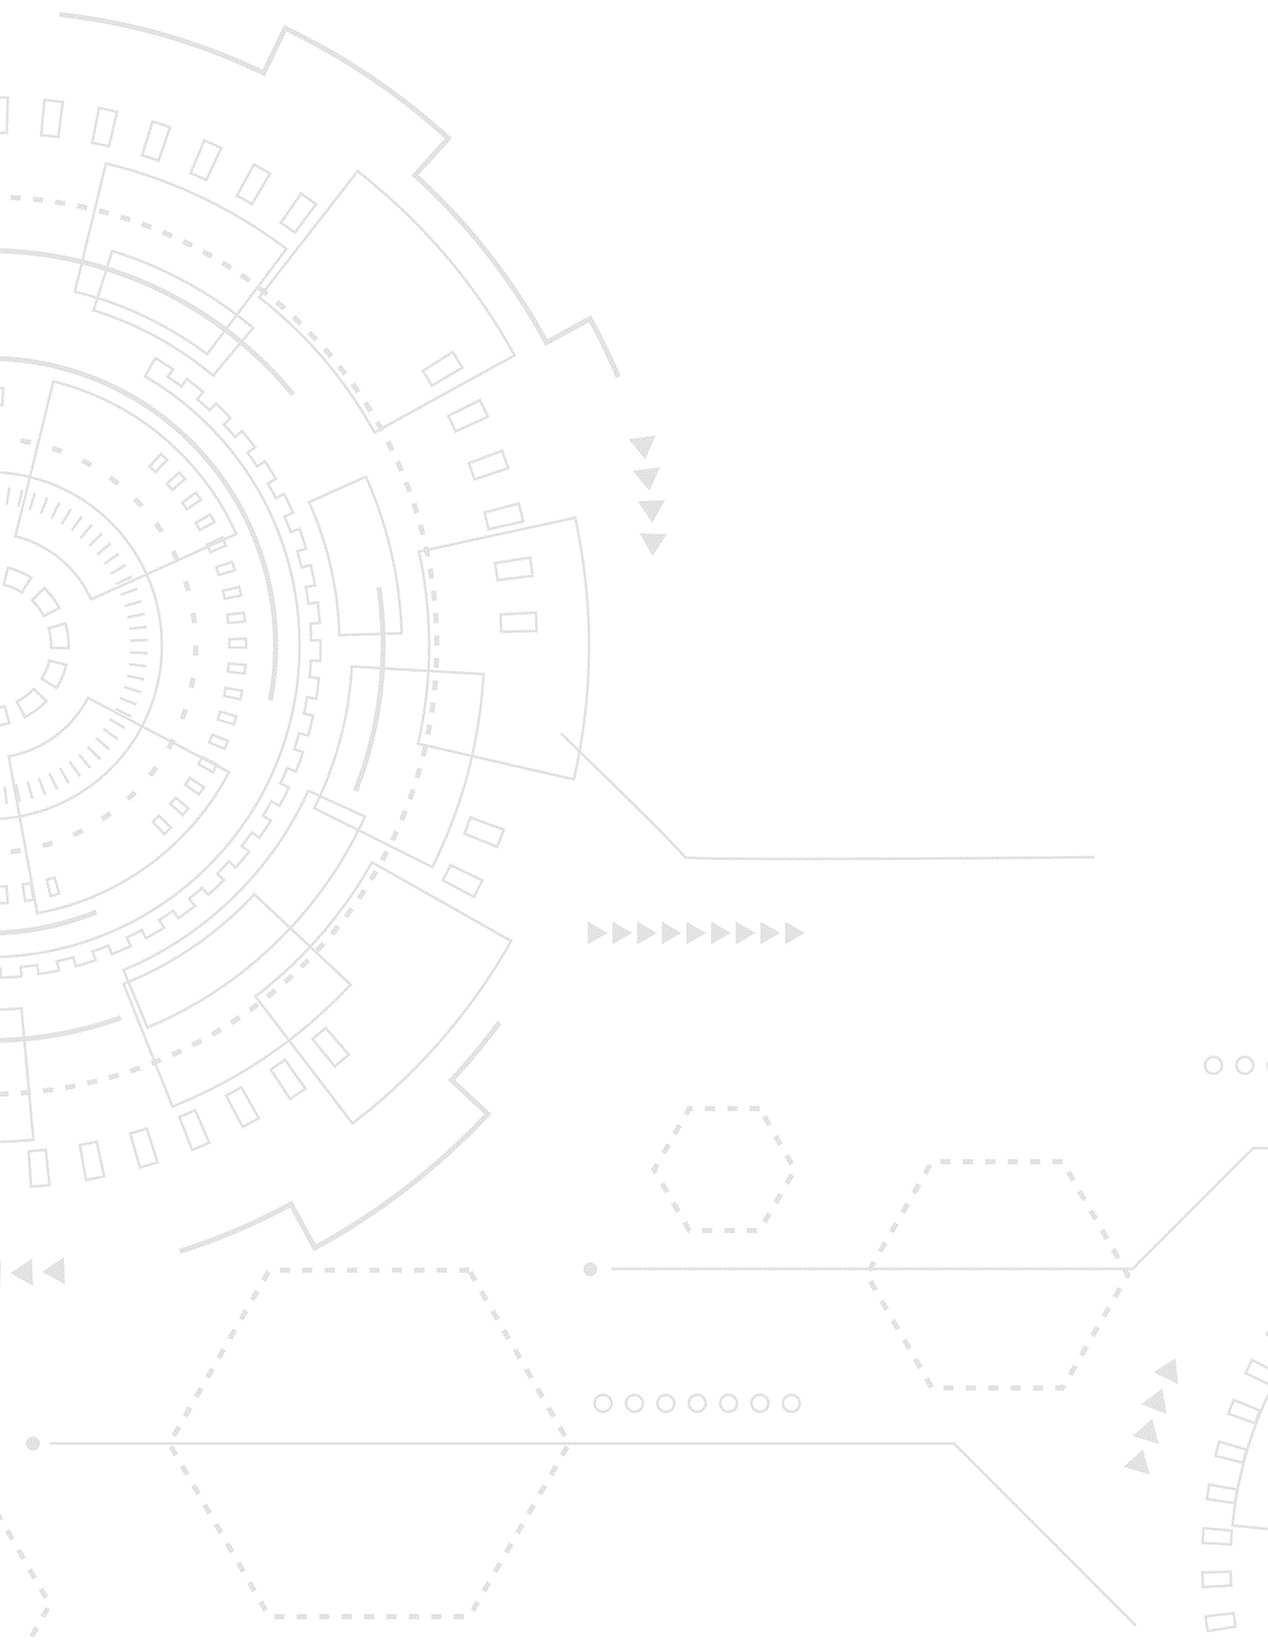
\includegraphics[width=\paperwidth,height=\paperheight]{mcdi.png}}}
\begin{center}
\vspace*{15em}
{\huge\bfseries\color{blue}{Capítulo 1}\par}
{\huge\bfseries\color{blue}{Los Datos y el Problema}\par}
\end{center}
%------------------------------------------
%Capítulo 1
%------------------------------------------
\chapter{Capítulo 1}
\gls{latex}
Hello\index{hello} world\index{world}!~\cite{Carpizo1998}

Ejemplo de cita. \cite{Kelsen1969}

Otro ejemplo de cita. \cite{Castro1998}
%----------------------------
% Subtítulo
%----------------------------
\section{Identificación de las fuentes de datos}
%----------------------------
% Contenido
Para la investigación, se ocupará el dataset Enron-Spam.
El dataset Enron-Spam es un conjunto de correos electrónicos utilizado principalmente para el entrenamiento de algoritmos de filtro de spam y análisis de texto. La historia de este conjunto de datos se remonta al escándalo de contabilidad de la compañía Enron, una empresa de energía que colapsó en 2001.

Durante la investigación realizada por el Departamento de Justicia de los Estados Unidos, se recolectaron una gran cantidad de correos electrónicos de la empresa, incluidos correos electrónicos personales y de negocios. En total, el conjunto de datos Enron-Spam está compuesto por alrededor de 500,000 correos electrónicos, con una mezcla de correos legítimos y spam.

Las características del conjunto de datos Enron-Spam incluyen la gran cantidad de correos electrónicos disponibles, lo que lo hace una opción popular para la investigación de filtrado de spam y análisis de texto. Además, los correos electrónicos fueron escritos en un entorno empresarial, lo que los hace diferentes de los correos electrónicos personales y redes sociales.

Entre las ventajas del conjunto de datos Enron-Spam, destaca la posibilidad de entrenar algoritmos de filtrado de correo no deseado con una gran cantidad de datos y con correos electrónicos de una fuente real y variada. Además, estos correos electrónicos se escribieron usando una variedad de estilos de escritura y cubren una amplia gama de temas, lo que hace que sea un conjunto de datos desafiante e interesante para análisis.

Entre las desventajas del conjunto de datos Enron-Spam, destaca su tamaño, ya que al ser muy grande, puede ser difícil trabajar con él en algunas herramientas y plataformas. Asimismo, los correos electrónicos están marcados como legítimos o spam, pero no tienen etiquetas adicionales que los clasifiquen en términos de contenido o intenciones específicas.

Muchas investigaciones han utilizado el conjunto de datos Enron-Spam en sus estudios, principalmente en las áreas de aprendizaje automático, minería de datos y análisis de texto. Los resultados de estas investigaciones han permitido la mejora de los sistemas de filtrado de correo no deseado para proporcionar a los usuarios una experiencia más óptima en el uso del correo electrónico.

En síntesis, el conjunto de datos Enron-Spam es un conjunto de correo electrónico amplio, útil y desafiante para la investigación relacionada con el spam en correo electrónico y el análisis de texto. Además, la fuente real y legítima de los correos electrónicos lo convierte en una excelente opción para el entrenamiento de algoritmos de filtro de correo electrónico.	
%----------------------------
\section{Planteanimiento del problema}
%----------------------------
% Contenido
El Aprendizaje Computacional o Machine Learning puede contribuir a detectar los mensajes de spam. Representa un verdadero reto, porque la variedad de los tipos de mensajes de este tipo es inmesa, pero la aplicación de aprendizaje profundo y otros métodos de IA (Inteligencia Artificial) puede contribuir a la correcta clasificación de este tipo de mensajes con una aceptación significativa. Se llevará a cabo un anális comparativo de  algunos de los algoritmos que se han utilizado para lograr este objetivo.
%----------------------------
\section{Preguntas, hipótesis y objetivos}
%----------------------------
% Contenido
Objetivo General
Comparar algunos de los algoritmos de Aprendizaje Automático para la clasificación de mensajes de spam. Al concluir el estudio comparativo de algoritmos de Aprendizaje Automático para la clasificación de spam en mensajes de correo electrónico, pretendo contar con datos suficientes para poder sacar conclusiones en cuanto a la utilidad relativa de cada algoritmo.
Objetivos Específicos
1. Revisar los estudios comparativos de algoritmos de Aprendizaje Automático para la clasificación de mensajes de spam que se han llevado a cabo, para seleccionar los más efectivos.
2. Examinar algoritmos de Aprendizaje Automático que se hayan utilizado para la solución de otros problemas, pero que pudieran servir también para la clasificación de mensajes de spam.
3. Realizar un estudio comparativo de algoritmos de Aprendizaje Automático para la clasificación de mensajes de spam, que incluya los seleccionados a partir del logro de los 2 primeros objetivos.
%----------------------------
\section{Creación de la base de datos}
%----------------------------
% Contenido
La base de datos es un conjunto de correos electrónicos clasificados como spam o ham (no spam). Se trata de 17,171 mensajes de spam y 16,545 mensajes de ham. El tipo de datos es texto, consistente en el asunto y el cuerpo del mensaje de correos electrónicos en inglés.
%----------------------------
